% ----------------------------------------------------------------- %
%             The Speech Signal Processing Toolkit (SPTK)           %
%             developed by SPTK Working Group                       %
%             http://sp-tk.sourceforge.net/                         %
% ----------------------------------------------------------------- %
%                                                                   %
%  Copyright (c) 1984-2007  Tokyo Institute of Technology           %
%                           Interdisciplinary Graduate School of    %
%                           Science and Engineering                 %
%                                                                   %
%                1996-2012  Nagoya Institute of Technology          %
%                           Department of Computer Science          %
%                                                                   %
% All rights reserved.                                              %
%                                                                   %
% Redistribution and use in source and binary forms, with or        %
% without modification, are permitted provided that the following   %
% conditions are met:                                               %
%                                                                   %
% - Redistributions of source code must retain the above copyright  %
%   notice, this list of conditions and the following disclaimer.   %
% - Redistributions in binary form must reproduce the above         %
%   copyright notice, this list of conditions and the following     %
%   disclaimer in the documentation and/or other materials provided %
%   with the distribution.                                          %
% - Neither the name of the SPTK working group nor the names of its %
%   contributors may be used to endorse or promote products derived %
%   from this software without specific prior written permission.   %
%                                                                   %
% THIS SOFTWARE IS PROVIDED BY THE COPYRIGHT HOLDERS AND            %
% CONTRIBUTORS "AS IS" AND ANY EXPRESS OR IMPLIED WARRANTIES,       %
% INCLUDING, BUT NOT LIMITED TO, THE IMPLIED WARRANTIES OF          %
% MERCHANTABILITY AND FITNESS FOR A PARTICULAR PURPOSE ARE          %
% DISCLAIMED. IN NO EVENT SHALL THE COPYRIGHT OWNER OR CONTRIBUTORS %
% BE LIABLE FOR ANY DIRECT, INDIRECT, INCIDENTAL, SPECIAL,          %
% EXEMPLARY, OR CONSEQUENTIAL DAMAGES (INCLUDING, BUT NOT LIMITED   %
% TO, PROCUREMENT OF SUBSTITUTE GOODS OR SERVICES; LOSS OF USE,     %
% DATA, OR PROFITS; OR BUSINESS INTERRUPTION) HOWEVER CAUSED AND ON %
% ANY THEORY OF LIABILITY, WHETHER IN CONTRACT, STRICT LIABILITY,   %
% OR TORT (INCLUDING NEGLIGENCE OR OTHERWISE) ARISING IN ANY WAY    %
% OUT OF THE USE OF THIS SOFTWARE, EVEN IF ADVISED OF THE           %
% POSSIBILITY OF SUCH DAMAGE.                                       %
% ----------------------------------------------------------------- %
\hypertarget{glogsp}{}
\name{glogsp}{draw a log spectrum graph}{plotting graphs}

\begin{synopsis}
\item[glogsp] [ --F $F$] [ --O $O$ ] [ --x $X$ ] [ --y $ymin \; ymax$ ] [ --ys $YS$ ] 
              [ --p $P$ ] [ --ln $LN$ ] 
\item[\ ~~~~~~~] [ --s $S$ ] [ --l $L$ ] [ --c $comment$ ] [ {\em infile} ]
\end{synopsis}

\begin{qsection}{DESCRIPTION}
{\em glogsp} converts float-format log spectral data 
from {\em infile} (or standard input)
to FP5301 plot format, 
sending the result to standard output. 
The output can be visualized with \hyperlink{xgr}{xgr}.

{\em glogsp} is implemented as a shell script 
that uses the \hyperlink{fig}{fig} and \hyperlink{fdrw}{fdrw} commands.
\end{qsection}

\begin{options}
        \argm{F}{F}{factor}{1}
	\argm{O}{O}{origin of graph\\
		      \begin{minipage}{4.5cm}
		       \begin{tabular}{ccc}
			1 & ( 40,205) & [mm] \\
			2 & (125,205) & [mm] \\
			3 & ( 40,120) & [mm] \\
			4 & (125,120) & [mm] \\
			5 & ( 40, 35) & [mm] \\
			6 & (125, 35) & [mm]
		       \end{tabular}\\\hspace*{\fill}
		      \end{minipage}
		      \begin{minipage}{4.5cm}
		       \leavevmode
		       \includegraphics{fig/glogsp-on.eps}
		      \end{minipage}\\\hspace*{\fill}}{1}
	\argm{x}{X}{ $x$ scale\\
		       \begin{tabular}{cl}
			1 & normalized frequency ($0 \sim 0.5$) \\
			2 & normalized frequency ($0 \sim \pi$) \\
			4 & frequency ($0 \sim 4$ kHz) \\
			5 & frequency ($0 \sim 5$ kHz) \\
			8 & frequency ($0 \sim 8$ kHz) \\
			10 & frequency ($0 \sim 10$ kHz) 
		       \end{tabular}\\\hspace*{\fill}}{1}
	\argm{y}{ymin \; ymax}{ $y$ scale[dB]}{0 100}
	\argm{ys}{YS}{ Y-axis scaling factor}{20}
	\argm{p}{P}{pen number($1 \sim 10$)}{1}
	\argm{ln}{LN}{kind of line style($0 \sim 5$) (see also \hyperlink{fig}{fig})}{1}
	\argm{s}{S}{start frame number}{0}
	\argm{l}{L}{frame length}{256}
	\argm{c}{\rm comment}{comment for the graph}{N/A}
	\desc[1ex]{Usually, the options below do not need to be assigned.}
	\argm{W}{W}{width of the graph ($\time 100$ mm)}{0.6}
	\argm{H}{H}{height of the graph ($\time 100$ mm)}{0.6}
	\argm{v}{}{over write mode}{FALSE}
	\argm{o}{xo \; yo}{origin of the graph.
                      if -o option exists, -O is not effective}{40 205}
	\argm{g}{G}{type of frame of the graph ($0 \sim 2$) (see also
	\hyperlink{fig}{fig})}{2}
	\argm{f}{file}{additional data file for \hyperlink{fig}{fig}}{NULL}
	\argm{help}{}{print help in detail}{}
\end{options}

\begin{qsection}{EXAMPLE}
In the example below, speech data sampled at 10 kHz is read
in short format from {\em data.s} file,
the magnitude of its log spectrum is evaluated and plotted on the screen:
\begin{quote}
 \verb!x2x +sf data.s | bcut +f -s 4000 -e 4255 | window -n 2| spec |\! \\
 \verb!glogsp -x 5 | xgr!
\end{quote}
\begin{center}
 \leavevmode
 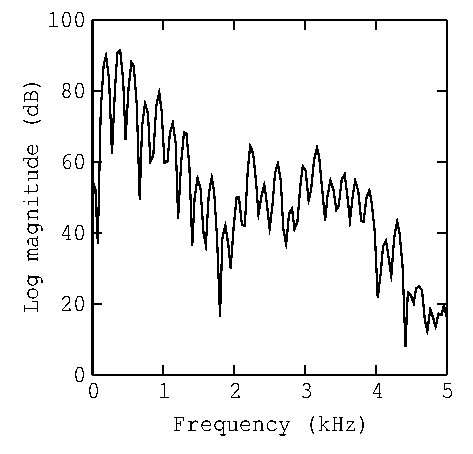
\includegraphics{fig/glogsp-sample.eps}
\end{center}
\end{qsection}

\begin{qsection}{SEE ALSO}
\hyperlink{fig}{fig},
\hyperlink{fdrw}{fdrw},
\hyperlink{xgr}{xgr},
\hyperlink{psgr}{psgr},
\hyperlink{grlogsp}{grlogsp},
\hyperlink{gwave}{gwave}
\end{qsection}

